\chapter{原子结构的描述}


在物理学中，处理复杂体系时，我们通常采用\textbf{按能量尺度逐级展开}的方法。这意味着，我们首先找出主导的相互作用项，然后再逐步引入较小的修正项。这种“分层近似”的思想，在原子结构理论中尤为常见。其实，原子哈密顿量在严格的形式下非常复杂，几乎不可能进行高精度计算，所以我们只能依赖实验来获取能级信息。因此，在实际处理中，我们需要对各相互作用的能量量级进行比较，判断哪些项是主导因素，哪些项可以视作微扰修正。这样，我们就能在实验精度的范围内较好地理解原子的行为。

以铷-87（$^{87}\text{Rb}$）原子的能级图为例，AMO实验的第一步就是搞懂这张图\ref{fig:appA-1}。

\begin{figure}[htbp]
	\centering
	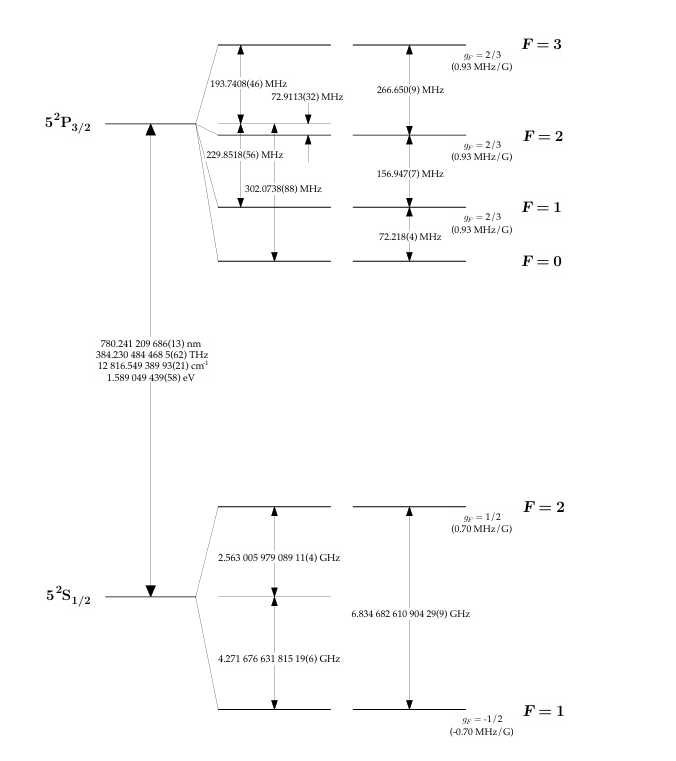
\includegraphics[width=0.6\linewidth]{figs/appB-1.png}
	\caption{铷-87（$^{87}\text{Rb}$）原子的D2线能级图}
	\label{fig:appA-1}
\end{figure}

原子哈密顿量一般可以写作：

\[
\hat{H} = \hat{H}_0 + \hat{H}_\text{SOC} + \hat{H}_\text{HFS} + \hat{H}_B,
\]

其中 $\hat{H}_0$ 是中心场近似下的主哈密顿量，$\hat{H}_\text{SOC}$ 是自旋—轨道耦合项，$\hat{H}_\text{HFS}$ 是超精细相互作用项，$\hat{H}_B$ 是外磁场相互作用项。不同项代表着不同的能量尺度，原子的能级结构正是通过逐步引入这些尺度而形成的。

如果不考虑外场作用，能量尺度最大的是 $\hat{H}_0$。以氢原子为例，当只考虑 $\hat{H}_0$ 时，能级只与主量子数 $n$ 有关。此时，$n,l,m_l$（以及电子自旋量子数 $s,m_s$）都是好量子数，其本征方程是：

\[
\hat{H}_0 \ket{n,l,m_l} = E_n \ket{n,l,m_l},
\]

\[
\hat{L}^2 \ket{n,l,m_l} = l(l+1)\hbar^2 \ket{n,l,m_l},
\]

\[
\hat{L}_z \ket{n,l,m_l} = m_l \hbar \ket{n,l,m_l}.
\]

由于库仑势的对称性，氢原子能级有很高的简并性，正是这种简并形成了我们熟悉的玻尔能级结构。氢原子基态的能量约为 $-13.6\ \text{eV}$，与第一激发态之间的能量差大约是几个eV。

我们研究的主要对象是碱金属原子。原子核与内层电子可等效成一个原子实，价电子与原子实的库仑相互作用构成能量的主项，其能级可表示为
\[
E_{nl} = - R_\infty h c \cdot \frac{1}{(n - \delta_{nl})^2},
\]
其中 $n$ 为主量子数，$\delta_{nl}$ 为量子数亏损。内层电子的存在屏蔽了一部分原子核的正电荷，使有效电荷趋近于1。角量子数 $l$ 越大，电子离原子实越远，屏蔽效果越好，故 $\delta_{nl}$ 越小，如图\ref{fig:appA-2}。
\begin{figure}[htbp]
	\centering
	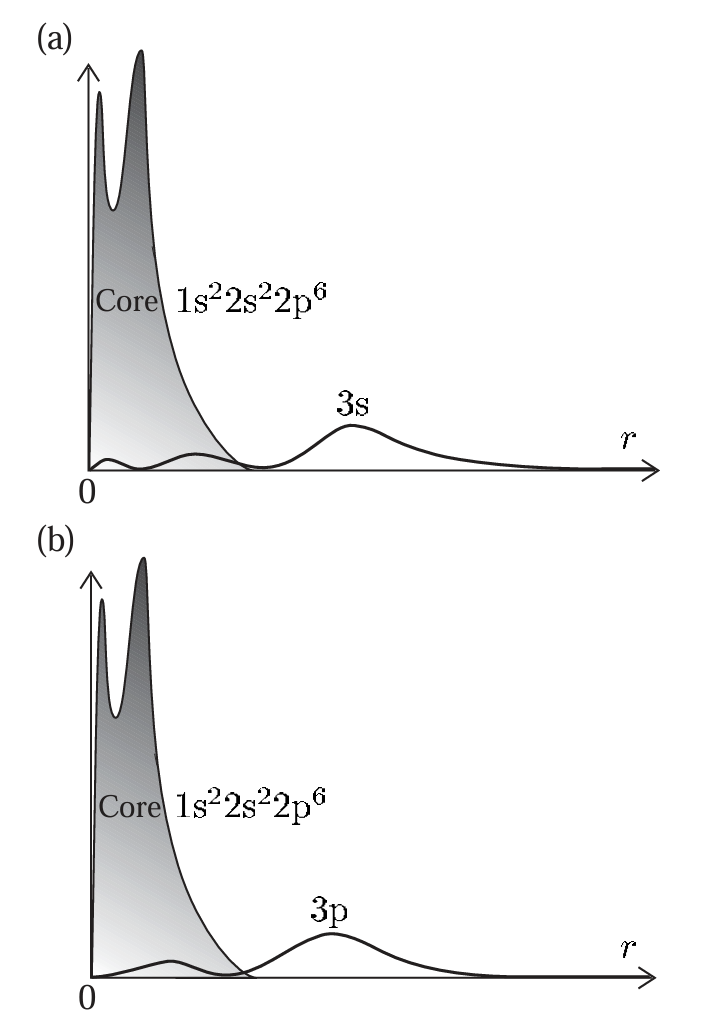
\includegraphics[width=0.3\linewidth]{figs/appB-3.png}
	\caption{不同角量子数 $l$的屏蔽效果}
	\label{fig:appA-2}
\end{figure}

因此，与主量子数相同的氢原子能级相比，碱金属原子的能级更低，这便是\textbf{量子数亏损理论}的核心结论。

对于常见的碱金属原子，它们的主项能量通常位于光学频段，量级大约为 $1\ \mathrm{eV}$。比如 $^{87}\mathrm{Rb}$ 的 $5S_{1/2}\rightarrow5P_{3/2}$ 跃迁的波长大约是 $780\ \mathrm{nm}$。

引入自旋—轨道耦合项 $\hat{H}_\text{SOC}$ 后，能级的简并性会部分解除，形成精细结构分裂。此时，轨道角动量 $\boldsymbol{L}$ 和自旋角动量 $\boldsymbol{S}$ 耦合成总角动量 $\boldsymbol{J}=\boldsymbol{L}+\boldsymbol{S}$，$m_l$ 和 $m_s$ 不再是好量子数，新的好量子数是 $n,l,s,j,m_j$，满足：

\[
\hat{J}^2 \ket{n,l,s,j,m_j} = j(j+1)\hbar^2 \ket{n,l,s,j,m_j},
\]

\[
\hat{J}_z \ket{n,l,s,j,m_j} = m_j \hbar \ket{n,l,s,j,m_j}.
\]

精细结构的能量尺度大约是主能级间隔的 $\alpha^2$（$\alpha$ 为精细结构常数）。我们最熟悉的双线结构就是钠的双黄线，其微小的能量分裂通常处于毫电子伏特（meV）量级。

如果再考虑超精细相互作用 $\hat{H}_\text{HFS}$，核自旋自由度会参与能级的决定。电子的总角动量 $\boldsymbol{J}$ 和核自旋 $\boldsymbol{I}$ 耦合成总角动量 $\boldsymbol{F}=\boldsymbol{I}+\boldsymbol{J}$，此时的好量子数是 $n,l,s,j,I,F,m_F$，满足：

\[
\hat{F}^2 \ket{n,l,s,j,I,F,m_F} = F(F+1)\hbar^2 \ket{n,l,s,j,I,F,m_F},
\]

\[
\hat{F}_z \ket{n,l,s,j,I,F,m_F} = m_F \hbar \ket{n,l,s,j,I,F,m_F}.
\]

超精细分裂的能量尺度比精细结构要小，通常在 GHz 到 MHz 的微波和射频频段。更高精度下，我们还可以观察到兰姆位移等微小的修正，但它们的量级更低，实验中通常不需要考虑。

到这里，我们就能完全理解铷-87的能级图。能级是否分裂完全取决于我们考虑的精度，耦合项的引入意味着两个独立的角动量开始耦合。

从角动量的角度看，这个过程展示了角动量逐步耦合的结构。对于两个独立的角动量 $\boldsymbol{J}_1$ 和 $\boldsymbol{J}_2$，如果它们没有耦合，系统的状态就可以用直积基 $\ket{j_1,m_1}\ket{j_2,m_2}$ 描述；而当它们耦合成总角动量 $\boldsymbol{J}$ 时，应该使用耦合基 $\ket{j_1,j_2;J,M}$ 来描述，二者之间通过 Clebsch–Gordan 系数相联系：

\[
\ket{j_1,j_2;J,M} = \sum_{m_1,m_2} \langle j_1,j_2;m_1,m_2 \vert J,M \rangle \ket{j_1,j_2;m_1,m_2}.
\]

需要注意的是，角动量耦合的方式实际上是由不同相互作用的能量尺度决定的。当某个相互作用远小于主导项时，我们可以把它看作微扰项；而当外加的磁场或电场足够强时，能量尺度的排序会发生变化，体系可能进入强场极限（比如 Paschen–Back 区域），此时原有的耦合近似会失效，角动量也会重新解耦。

因此，分析原子能级结构，本质上是一个根据能量层级逐步展开并不断修正对称性结构的过程。

AMO实验中另一张常用的示意图是塞曼分裂图\ref{fig:appA-3}。

\begin{figure}[htbp]
	\centering
	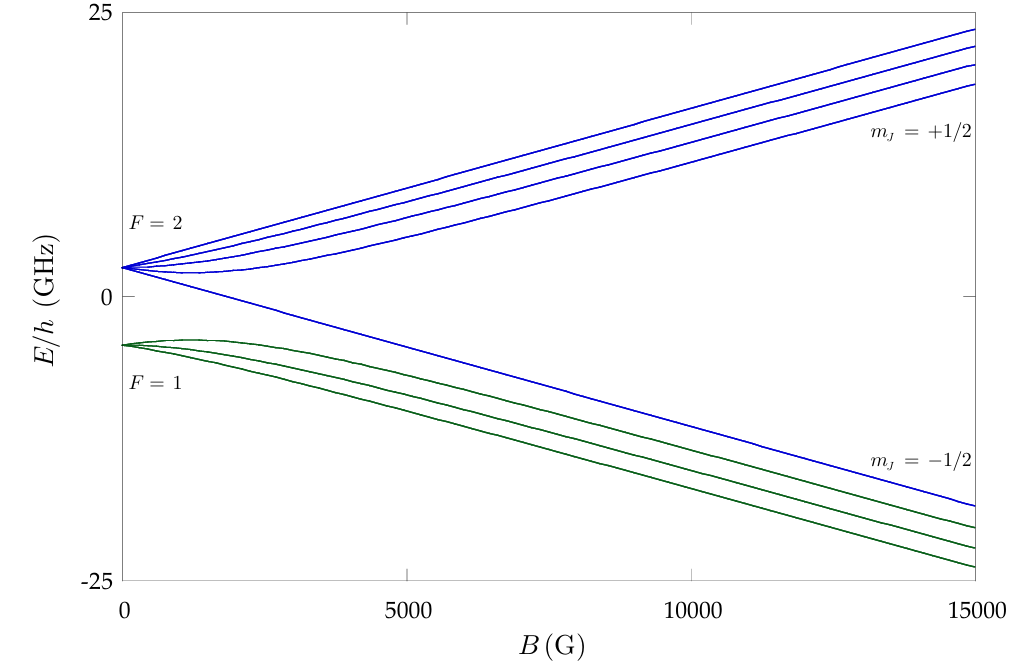
\includegraphics[width=0.6\linewidth]{figs/appB-2.png}
	\caption{铷-87（$^{87}\text{Rb}$）原子的基态塞曼分裂图}
	\label{fig:appA-3}
\end{figure}

在小磁场情况下，$\Delta E_B \ll \Delta E_\text{HFS}$，$\hat{H}_B$ 被当成微扰处理，$I$ 和 $J$ 依然耦合，$m_F$ 仍然是“好”量子数，能级仍然可以用$\ket{n,l,s,j,I,F,m_F}$ 来描述。因此：

\[
\Delta E_B = m_F g_F \mu_B B_z
\]

在弱磁场下，$m_F g_F$ 的符号决定了线性分裂的方向。$m_F = 0$ 的态对磁场不敏感，通常作为\textbf{钟跃迁态}。

在强磁场（Paschen–Back 区域）下，$\Delta E_B \gg \Delta E_\text{HFS}$，$\hat{H}_B$ 不再是微扰，$\hat{H}_\text{HFS}$ 可以被忽略，$I$ 和 $J$ 会解耦，能级用$\ket{n,l,s,j,m_j,I,m_I}$ 来描述，因此，$I$ 和 $J$ 会决定能级分裂的大小和方向。强磁场下，能量分裂的公式为：

\[
\Delta E_B = \dots + \mu_B \bigl( g_J m_J + g_I m_I \bigr) B_z
\]

其中 $g_I \approx -10^{-3}$，而 $g_J \approx 1$。因此，能级分裂的方向主要由 $m_J$ 的符号和大小决定。在强磁场下，$m_J$ 为正的能级会上升，$m_J$ 为负的能级则会下降。

磁光阱和磁阱的理论基础正是基于这个原理，而丰富的内态也为能级操控提供了更多的可能，附录B将介绍辐射场与原子的相互作用。